\documentclass[11pt]{article}
\usepackage[a4paper,left=1.5cm,right=1.5cm,top=1.5cm,bottom=1.5cm]{geometry}
\usepackage{fancyhdr}
\renewcommand{\headrulewidth}{1pt}
\fancyhead[C]{\textbf{[LINMA1170] SVD et conditionnement}}
\fancyhead[L]{Novembre 2018}
\fancyhead[R]{Gilles Peiffer [24321600]}

\usepackage[T1]{fontenc}
\usepackage[utf8]{inputenc}
\usepackage[french]{babel}
\usepackage{graphicx}
\usepackage{subcaption}
\usepackage{mathtools,amssymb}
\usepackage[binary-units=true,separate-uncertainty = true,multi-part-units=single]{siunitx}
\usepackage{float}
\usepackage[linktoc=all]{hyperref}
\hypersetup{breaklinks=true}
\setlength{\parindent}{0cm}
\setlength{\parskip}{1ex plus 0.5ex minus 0.2ex}
\newcommand{\hsp}{\hspace{20pt}}
\newcommand{\HRule}{\rule{\linewidth}{0.5mm}}
\graphicspath{{img/}}
\usepackage{caption}
\usepackage{textcomp}
\usepackage{array}
\usepackage{color}
\usepackage{tabularx,booktabs}
\usepackage{titlesec}
\titlespacing{\section}{0pt}{\parskip}{-\parskip}
\titlespacing{\subsection}{0pt}{\parskip}{-\parskip}
\titlespacing{\subsubsection}{0pt}{\parskip}{-\parskip}
\pagestyle{fancy}
\DeclarePairedDelimiterX{\norm}[1]{\lVert}{\rVert}{#1}

\begin{document}
\section{Paramètres influençant le conditionnement de $A$}
\subsection{Largeur de l'entrefer}
Moins l'entrefer est large, plus le maillage doit être raffiné à cet endroit.
Nous remarquons donc que pour de petites valeurs,
le conditionnement de la matrice 
\subsection{Perméabilité relative du noyau magnétique}
\subsection{Courant injecté dans la bobine}
Le courant injecté dans la bobine n'est qu'un simple facteur multiplicatif dans les calculs.
Il n'intervient donc pas dans le conditionnement de la matrice, qui reste constant.
%TODO vérifier si le spectre est bien translaté vers le haut
\subsection{Raffinement du maillage}
Afin de voir l'effet du raffinement du maillage sur le conditionnement de la matrice $A$, nous avons joué sur le paramètre \texttt{clscale} de \texttt{ccore.py}.
Plus celui-ci est petit, plus le maillage est fin.
%TODO explain why it goes down as the mesh gets more coarse

\section{Approximation de rang faible}
Nous cherchons à approximer la matrice $A \in \mathbb{R}^{m \times n}$ de rang $r$ par une somme de $\nu$ matrices de rang $1$ comme suit:
\[
A_{\nu} = \sum_{j=1}^{\nu} \sigma_{j} u_{j} v^*_{j}\,. 
\] 
Par le Théorème~5.8 pp. 35--36 dans le livre de référence, il est possible de démontrer que cette somme partielle capture l'énergie maximale possible de $A$, et ce autant pour la $2$-norme matricielle (avec laquelle nous travaillons) que pour la norme de Frobenius.
On définit alors l'erreur $e_{\nu}$ comme
\[
e_{\nu} = \frac{\norm{A - A_{\nu}}_2}{\norm{A}_2}\,.
\]
Il était demandé de répondre à trois questions concernant ces approximations.
\subsection{Influence du premier terme}
%TODO explain first term proportion
\subsection{Nombre de termes requis pour obtenir une précision donnée}
%TODO explain terms in function of system size
\subsection{Influence du conditionnement}
%TODO explain terms in function of condition number
\appendix
\section*{Appendices}
\section{Figures}
%TODO add figures
%TODO change figure names
\begin{figure}[H]
	\centering
	\begin{subfigure}{0.4\textwidth}
		\centering
		%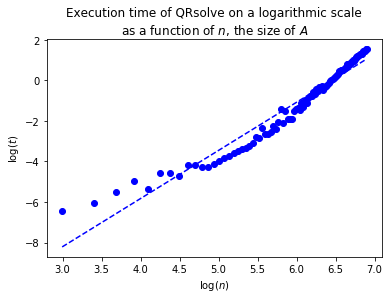
\includegraphics[width=\linewidth]{hw1_loglog_qr.png}
		\caption{\texttt{QRsolve}, échelle logarithmique.}
		\label{fig:llqr}
	\end{subfigure}%
	\begin{subfigure}{0.4\textwidth}
		\centering
		%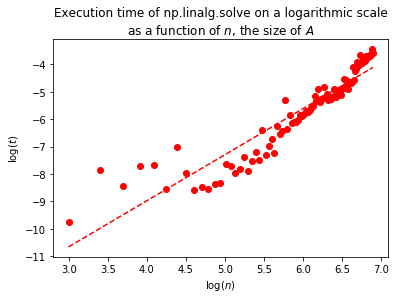
\includegraphics[width=\linewidth]{hw1_loglog_np.png}
		\caption{\texttt{NumPy}, échelle logarithmique.}
		\label{fig:llnp}
	\end{subfigure}
	\begin{subfigure}{0.4\textwidth}
		\centering
		%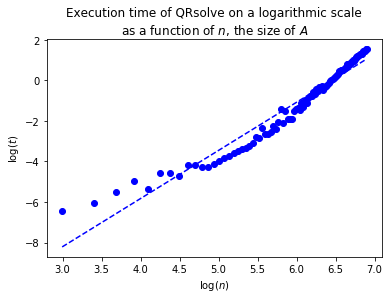
\includegraphics[width=\linewidth]{hw1_loglog_qr.png}
		\caption{\texttt{QRsolve}, échelle logarithmique.}
		\label{fig:llqr}
	\end{subfigure}%
	\begin{subfigure}{0.4\textwidth}
		\centering
		%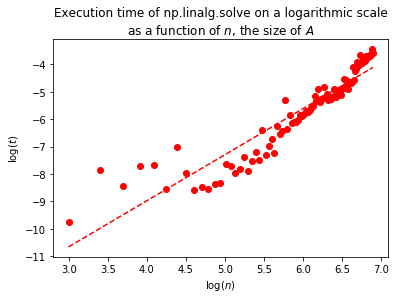
\includegraphics[width=\linewidth]{hw1_loglog_np.png}
		\caption{\texttt{NumPy}, échelle logarithmique.}
		\label{fig:llnp}
	\end{subfigure}
	\begin{subfigure}{0.4\textwidth}
		\centering
		%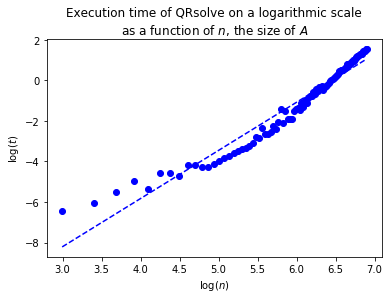
\includegraphics[width=\linewidth]{hw1_loglog_qr.png}
		\caption{\texttt{QRsolve}, échelle logarithmique.}
		\label{fig:llqr}
	\end{subfigure}%
	\begin{subfigure}{0.4\textwidth}
		\centering
		%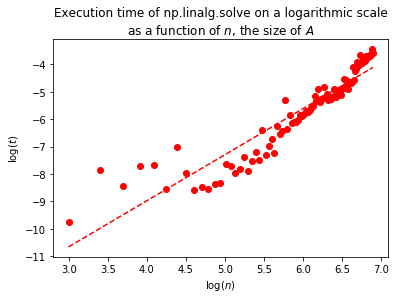
\includegraphics[width=\linewidth]{hw1_loglog_np.png}
		\caption{\texttt{NumPy}, échelle logarithmique.}
		\label{fig:llnp}
	\end{subfigure}
	\begin{subfigure}{0.4\textwidth}
		\centering
		%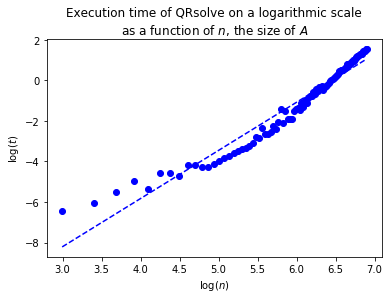
\includegraphics[width=\linewidth]{hw1_loglog_qr.png}
		\caption{\texttt{QRsolve}, échelle logarithmique.}
		\label{fig:llqr}
	\end{subfigure}%
	\begin{subfigure}{0.4\textwidth}
		\centering
		%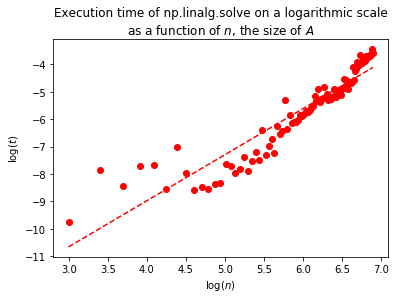
\includegraphics[width=\linewidth]{hw1_loglog_np.png}
		\caption{\texttt{NumPy}, échelle logarithmique.}
		\label{fig:llnp}
	\end{subfigure}
	\caption{Différents graphes pertinents pour l'analyse en page 1.}
	\label{fig:manmade}
\end{figure}
\end{document}